\documentclass[12pt]{article}

\usepackage[a4paper, top=2cm, bottom=2cm, left=2.2cm, right=2.2cm]{geometry}
\usepackage[T1]{fontenc}
\usepackage[utf8x]{inputenc}
\usepackage{lmodern}
\usepackage[spanish]{babel}
\usepackage{graphicx}
\usepackage{float}
\usepackage{multirow}
\usepackage{listings}

\author{LIDSOL Team :v}
\title{Pr\'actica 3}
\date{10 Abril del 2018}
\def\universidad{Universidad Nacional Aut\'onoma de M \'exico}
\def\facultad{Facultad de Ingenier\'ia}
\def\materia{Arquitectura de Computadoras}
\def\grupo{Grupo: 3}
\def\profesor{M.I. Jos\'e Luis Cruz Mora}
\def\luis{Oropeza Vilchis Luis Alberto}
\def\diego{Barriga Mart\'inez Diego Alberto}
\def\emilio{Cabrera L\'opez Oscar Emilio}
\makeatletter

\begin{document}
\pagenumbering{gobble}

% Escudos
\begin{figure}
	\begin{flushleft}
		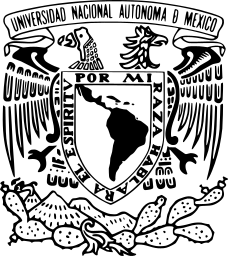
\includegraphics[width=3cm]{unam}\hfill 				
\includegraphics[width=3cm]{fi2}
	\end{flushleft}
\end{figure}

\begin{center}
	\Huge \universidad \\
	\hfill \\
	\facultad \\
	\hfill \\
    \materia\par
    \hfill \\
    \@title\par
    \hfill \\
    \profesor\par
    \hfill \\
    Integrantes:
    \hfill \\
    \hfill \\
    \diego \\
    \emilio \\
    \luis \\
    \hfill \\
    \grupo \\
    \hfill \\
    \@date \\
\end{center}

\newpage
\pagenumbering{arabic}

\section{Direccionamiento Entrada-Estado}

\begin{figure}[H]
	\centering
	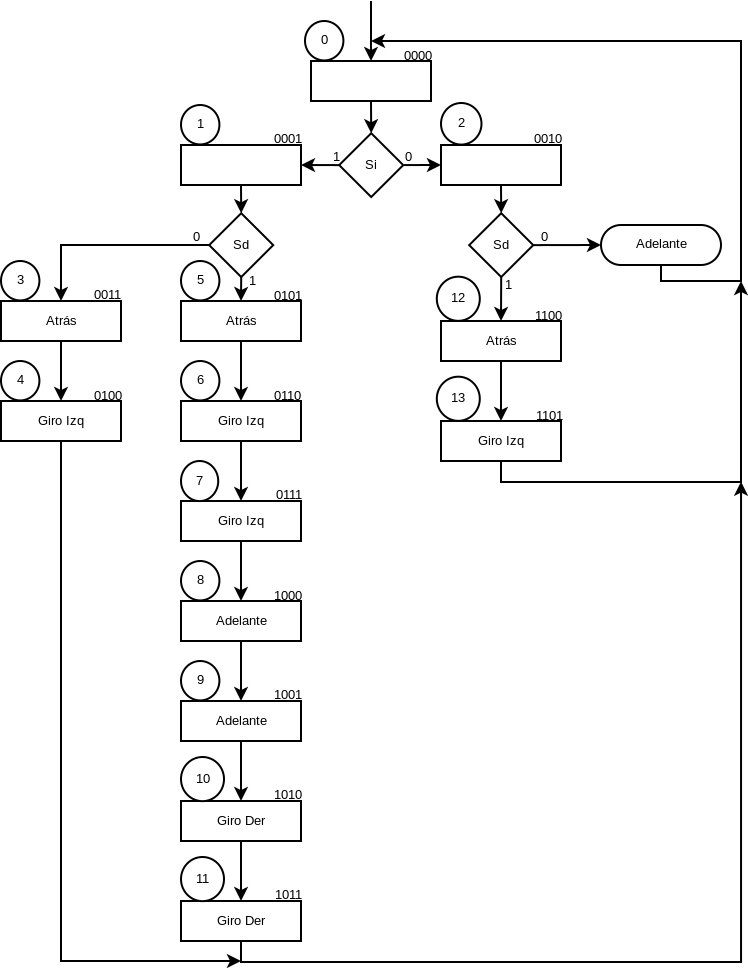
\includegraphics[width=0.8\textwidth]{carta_asm}
	\caption{Carta ASM modificada}
\end{figure}

\medskip
\noindent \textbf{N\'umero de estados:} 14, por lo que se utilizan 4 bits para representarlos\\
\textbf{Entradas:} $S_{i}$ y $S_{d}$\\
\textbf{Salidas:} Adelante (Ad), Atr\'as (At), Giro Izquierda (GI), Giro Derecha (GD)\\
\textbf{Prueba}:\\

\begin{center}
	\begin{tabular}{|c|c|}
		\hline
		 Entrada & C\'odigo\\
		\hline 
		$S_{i}$ & 0 0 \\ 
		\hline 
		$S_{d}$ & 0 1 \\ 
		\hline 
		$\uparrow Aux$ & 1 1 \\ 
		\hline 
	\end{tabular}\\
\end{center}

\noindent \textbf{ Contenido de la memoria:}\\
\begin{center}
	\begin{tabular}{|c|c|c|c|c|c|c|}
		\hline 
		\multicolumn{2}{|c|}{ \multirow{2}{*}{Estado}} & \multirow{2}{*}{Prueba} & \multirow{2}{*}{LV} & \multirow{2}{*}{LF} & SV & SF \\ 
		\cline{6-7}
		 \multicolumn{2}{|c|}{}& & & &Ad At GI GD & Ad At GI GD \\ 
		\hline 
		0   & 0 0 0 0 & 0 0 & 0 0 0 1 & 0 0 1 0 & 0 0 0 0 & 0 0 0 0 \\ 
		\hline                                                     
		1   & 0 0 0 1 & 0 1 & 0 1 0 1 & 0 0 1 1 & 0 0 0 0 & 0 0 0 0 \\ 
		\hline                                                     
		2   & 0 0 1 0 & 0 1 & 1 1 0 0 & 0 0 0 0 & 0 0 0 0 & 1 0 0 0 \\ 
		\hline                                                     
		3   & 0 0 1 1 & 1 1 & 0 1 0 0 & 0 1 0 0 & 0 1 0 0 & 0 1 0 0 \\ 
		\hline                                                     
		4   & 0 1 0 0 & 1 1 & 0 0 0 0 & 0 0 0 0 & 0 0 0 1 & 0 0 0 1 \\ 
		\hline                                                     
		5   & 0 1 0 1 & 1 1 & 0 1 1 0 & 0 1 1 0 & 0 1 0 0 & 0 1 0 0 \\ 
		\hline                                                     
		6   & 0 1 1 0 & 1 1 & 0 1 1 1 & 0 1 1 1 & 0 0 1 0 & 0 0 1 0 \\ 
		\hline                                                     
		7   & 0 1 1 1 & 1 1 & 1 0 0 0 & 1 0 0 0 & 0 0 1 0 & 0 0 1 0 \\ 
		\hline                                                     
		8   & 1 0 0 0 & 1 1 & 1 0 0 1 & 1 0 0 1 & 1 0 0 0 & 1 0 0 0 \\ 
		\hline                                                     
		9   & 1 0 0 1 & 1 1 & 1 0 1 0 & 1 0 1 0 & 1 0 0 0 & 1 0 0 0 \\ 
		\hline                                                     
		10  & 1 0 1 0 & 1 1 & 1 0 1 1 & 1 0 1 1 & 0 0 0 1 & 0 0 0 1 \\ 
		\hline                                                     
		11  & 1 0 1 1 & 1 1 & 0 0 0 0 & 0 0 0 0 & 0 0 0 1 & 0 0 0 1 \\ 
		\hline                                                     
		12  & 1 1 0 0 & 1 1 & 1 1 0 1 & 1 1 0 1 & 0 1 0 0 & 0 1 0 0 \\ 
		\hline                                                     
		13  & 1 1 0 1 & 1 1 & 0 0 0 0 & 0 0 0 0 & 0 0 1 0 & 0 0 1 0 \\ 
		\hline 
	\end{tabular} 
\end{center}

\textbf{C\'odigo:}\\

\textit{Para la m\'aquina de estados:}
\begin{lstlisting}
library ieee;
use ieee.numeric_std.all;
use ieee.std_logic_1164.all;

entity entrada_estado is
	Port (
			reloj: in std_logic;
			entradas: in unsigned(1 downto 0); -- Bit menos significativo representa Si, else Sd
			salidas: out unsigned(3 downto 0)
			);
end entity;

architecture Behavioral of entrada_estado is
signal prueba: unsigned(1 downto 0);
signal sv, sf, lf, lv, salidas_mem, registro_mem, selector_liga, selector_salidas: unsigned(3 downto 0);
signal selector_entradas: std_logic;
signal mem_salida : unsigned(17 downto 0);

begin

-- Instancia de la memoria
memoria: entity work.memoria_ee
	port map(
		direccion => to_integer(registro_mem),
		salidas => mem_salida
	);

-- Multiplexor que elige la entrada
mux_entradas: selector_entradas <= entradas(0) when prueba = "00" else
											  entradas(1) when prueba = "01" else
											  '1';
-- Multiplexor que elige entre liga falsa y verdadera
mux_liga: selector_liga <= lf when selector_entradas = '0' else lv;
-- Multiplexor que elige entre salidas verdaderas o falsas
mux_salidas: selector_salidas <= sf when selector_entradas = '0' else sv;

-- Asignaciones de la salida de la memoria
-- Salidas falsa y verdadera
sf <= mem_salida(3 downto 0);
sv <= mem_salida(7 downto 4);
-- Liga falsa y verdadera
lf <= mem_salida(11 downto 8);
lv <= mem_salida(15 downto 12);
-- Prueba
prueba <= mem_salida(17 downto 16);

-- Registro que direcciona la memoria
reg_mem: process(reloj)
begin
	if rising_edge(reloj) then
		registro_mem <= selector_liga;
	end if;
end process;

-- Registro de las salidas
reg_salida: process(reloj)
begin
	if rising_edge(reloj) then
		salidas <= selector_salidas;
	end if;
end process;

end Behavioral;
\end{lstlisting}

\bigskip
\textit{Para la memoria:}
\begin{lstlisting}

library ieee;
use ieee.std_logic_1164.all;
use ieee.numeric_std.all;

entity memoria_ee is

	generic 
	(
		TAM_PALABRA : natural := 18;
		TAM_MEMORIA : natural := 14
	);

	port 
	(
		direccion	: in natural range 0 to 2**TAM_MEMORIA - 1;
		salidas		: out unsigned((TAM_PALABRA -1) downto 0)
	);

end entity;

architecture rtl of memoria_ee is
	subtype palabra_t is unsigned((TAM_PALABRA-1) downto 0);
	type memoria_t is array(TAM_MEMORIA-1 downto 0) of palabra_t;
	
	signal mem : memoria_t := (
		0 =>  "000001001000000000",
		1 =>  "010101001100000000",
		2 =>  "011100000000001000",
		3 =>  "110100010001000100",
		4 =>  "110000000000010001",
		5 =>  "110110011001000100",
		6 =>  "110111011100100010",
		7 =>  "111000100000100010",
		8 =>  "111001100110001000",
		9 =>  "111010101010001000",
		10 => "111011101100010001",
		11 => "110000000000010001",
		12 => "111101110101000100",
		13 => "110000000000100010"
	);
begin
	salidas <= mem(direccion);
end rtl;

\end{lstlisting}
\bigskip
\textbf{Simulaci\'on:}

\begin{figure}[H]
	\centering
	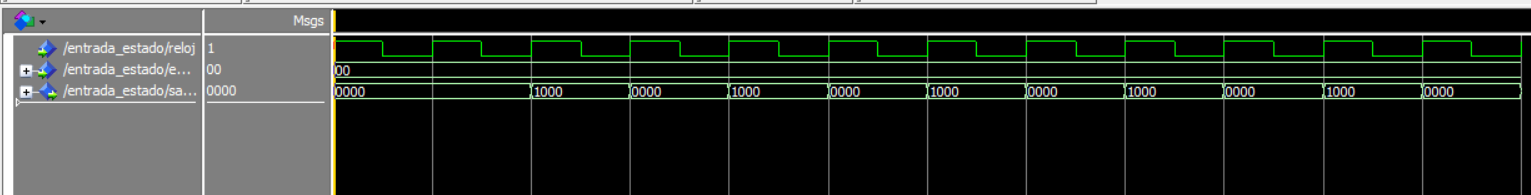
\includegraphics[width=1.0\textwidth]{input_00_ee}
	\caption{Entradas: 00}
\end{figure}

\begin{figure}[H]
	\centering
	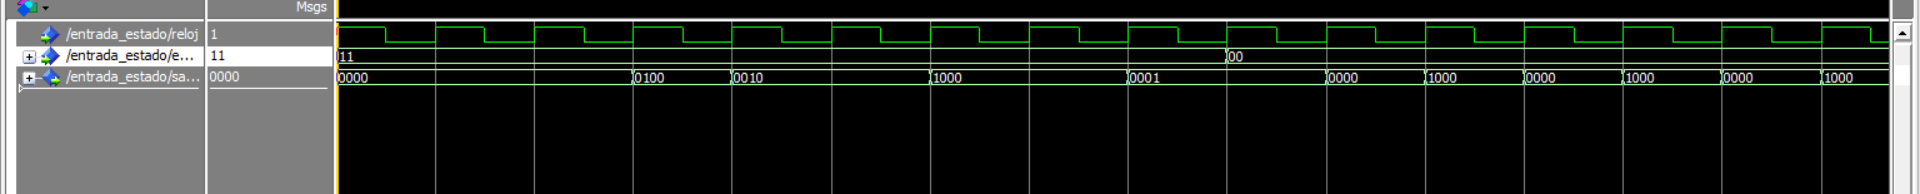
\includegraphics[width=1.0\textwidth]{input_11_ee}
	\caption{Entradas: 11}
\end{figure}

\newpage
\section{Direccionamiento Impl\'icito}

\begin{figure}[H]
	\centering
	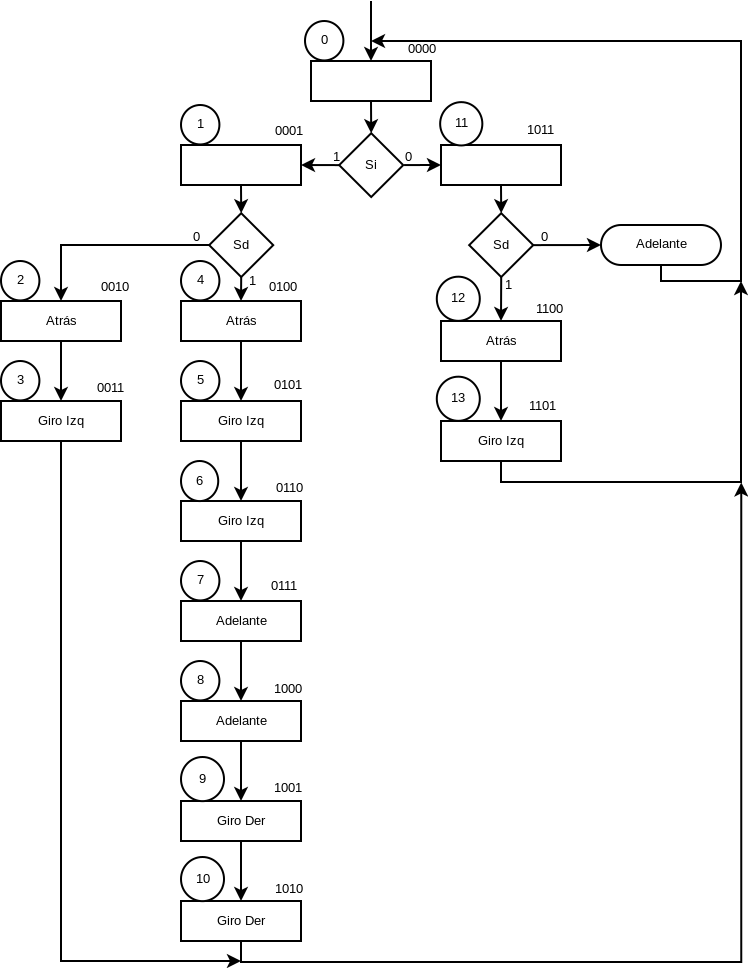
\includegraphics[width=0.8\textwidth]{carta_asm_implicito}
	\caption{Carta ASM modificada}
\end{figure}

\noindent \textbf{N\'umero de estados:} 14, por lo que se utilizan 4 bits para representarlos\\
\textbf{Entradas:} $S_{i}$ y $S_{d}$\\
\textbf{Salidas:} Adelante (Ad), Atr\'as (At), Giro Izquierda (GI), Giro Derecha (GD)\\
\textbf{Prueba}:\\
\begin{center}
	\begin{tabular}{|c|c|}
		\hline
		 Entrada & C\'odigo\\
		\hline 
		$S_{i}$ & 0 0 \\ 
		\hline 
		$S_{d}$ & 0 1 \\ 
		\hline 
		$\uparrow Aux$ & 1 1 \\ 
		\hline 
	\end{tabular}
\end{center}

\newpage
\textbf{Carga:}\\
\begin{center}
	\begin{tabular}{|c|c|c|}
		\hline 
		Entrada & VF & Carga \\ 
		\hline 
		0 & 0 & 1 \\ 
		\hline 
		0 & 1 & 0 \\ 
		\hline 
		1 & 0 & 0 \\ 
		\hline 
		1 & 1 & 1 \\ 
		\hline 
	\end{tabular} 
\end{center}

\textbf{Contenido de la memoria:}\\

\begin{center}
	\begin{tabular}{|c|c|c|c|c|c|c|}
		\hline 
		\multicolumn{2}{|c|}{ \multirow{2}{*}{Estado}} & \multirow{2}{*}{Prueba} & \multirow{2}{*}{VF} & \multirow{2}{*}{Liga} & SV & SF \\ 
		\cline{6-7}
		 \multicolumn{2}{|c|}{}& & & &Ad At GI GD & Ad At GI GD \\ 
		\hline 
		0   & 0 0 0 0 & 0 0 & 0 & 1 0 1 1 & 0 0 0 0 & 0 0 0 0\\ 
		\hline                                               
		1   & 0 0 0 1 & 0 1 & 1 & 0 1 0 0 & 0 0 0 0 & 0 0 0 0\\ 
		\hline                                               
		2   & 0 0 1 0 & 1 1 & 1 & 0 0 1 1 & 0 1 0 0 & 0 1 0 0\\ 
		\hline                                               
		3   & 0 0 1 1 & 1 1 & 1 & 0 0 0 0 & 0 0 1 0 & 0 0 0 1\\ 
		\hline                                               
		4   & 0 1 0 0 & 1 1 & 1 & 0 1 0 1 & 0 1 0 0 & 0 1 0 0\\ 
		\hline                                               
		5   & 0 1 0 1 & 1 1 & 1 & 0 1 1 0 & 0 0 1 0 & 0 0 1 0\\ 
		\hline                                               
		6   & 0 1 1 0 & 1 1 & 1 & 0 1 1 1 & 0 0 1 0 & 0 0 1 0\\ 
		\hline                                               
		7   & 0 1 1 1 & 1 1 & 1 & 1 0 0 0 & 1 0 0 0 & 1 0 0 0\\ 
		\hline                                               
		8   & 1 0 0 0 & 1 1 & 1 & 1 0 0 1 & 1 0 0 0 & 1 0 0 0\\ 
		\hline                                               
		9   & 1 0 0 1 & 1 1 & 1 & 1 0 1 0 & 0 0 0 1 & 0 0 0 1\\ 
		\hline                                               
		10  & 1 0 1 0 & 1 1 & 1 & 0 0 0 0 & 0 0 0 1 & 0 0 0 1\\ 
		\hline                                               
		11  & 1 0 1 1 & 0 1 & 0 & 0 0 0 0 & 0 0 0 0 & 1 0 0 0\\ 
		\hline                                               
		12  & 1 1 0 0 & 1 1 & 1 & 1 1 0 1 & 0 1 0 0 & 0 1 0 0\\ 
		\hline                                               
		13  & 1 1 0 1 & 1 1 & 1 & 0 0 0 0 & 0 0 1 0 & 0 0 1 0\\ 
		\hline 
	\end{tabular} 
\end{center}

\textbf{C\'odigo:}

\begin{lstlisting}

library ieee;
  use ieee.std_logic_1164.all;
  use ieee.numeric_std.all;

entity practica6 is
  port (
    clock     : in  std_logic;
    entradas  : in  unsigned(1 downto 0);
    salidas   : out unsigned(3 downto 0)
  );
end entity;

architecture arch of practica6 is
  signal carga_s, vf_s, ent_s: std_logic;
  signal prueba_s: unsigned(1 downto 0);
  signal liga_s, salv_s, salf_s, dir_s: unsigned(3 downto 0);
  signal sal_mem_s: unsigned(14 downto 0);
begin
  cont_e: entity work.contador port map(
    clock => clock,
    data  => liga_s,
    load  => carga_s,
    count => dir_s
  );

  rom_e: entity work.rom port map(
    cs        => '1',
    addr      => dir_s,
    data_out  => sal_mem_s
  );

  reg_outv_p: process(clock) begin
    if rising_edge(clock) then
			salv_s <= sal_mem_s(7 downto 4);
		end if;
	end process;

  reg_outf_p: process(clock) begin
    if rising_edge(clock) then
			salf_s <= sal_mem_s(3 downto 0);
		end if;
	end process;

  prueba_s <= sal_mem_s(14 downto 13);
  vf_s     <= sal_mem_s(12);
  liga_s   <= sal_mem_s(11 downto 8);
  carga_s  <= ent_s xnor vf_S;

  with prueba_s select
    ent_s <=  entradas(0) when  "00",
              entradas(1) when  "01",
              '1'         when  "11",
              '1'         when  others;

  salidas <= salf_s when vf_s = '0' else salv_s;

end architecture;

\end{lstlisting}

\bigskip
\textbf{Simulaci\'on:}

\begin{figure}[H]
	\centering
	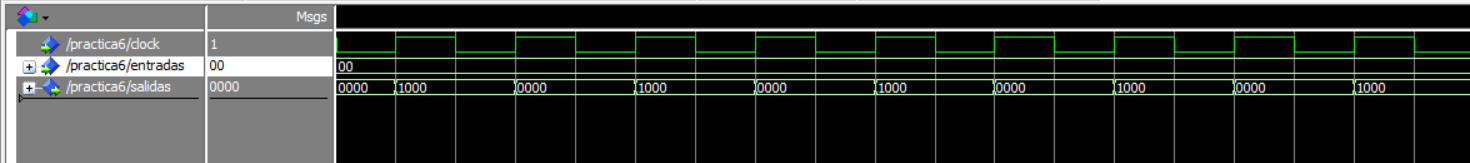
\includegraphics[width=1.0\textwidth]{input_00_imp}
	\caption{Entradas: 00}
\end{figure}

\begin{figure}[H]
	\centering
	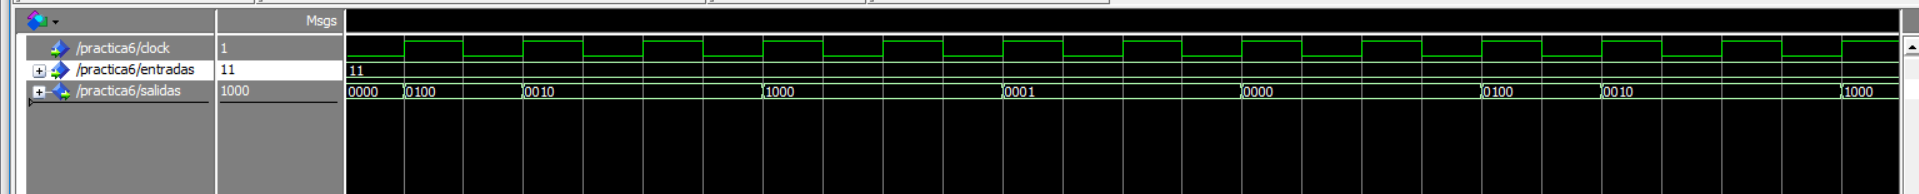
\includegraphics[width=1.0\textwidth]{input_11_imp}
	\caption{Entradas: 11}
\end{figure}

\section*{Conclusiones}

% Please, put your comments here
\subsection*{\diego}
La tercera pr\'actica se ha vuelto m\'as interesante ya que se sientan las bases con las que se trabajar\'a a lo largo del semestre. El uso de direccionamientos es ampliamente utilizado porque reduce repetici\'on y creaci\'on de tablas enormes de estados. Entrada-Estado y direccionamiento impl\'icito son buenos acercamientos a lo que m\'as adelante ser\'a el proyecto final que es mucho m\'as cercano a un proyecto real que los ejercicios en clase. Con esto y los constantes ejercicios y tareas se reafirma el entendimiento de los direccionamientos.
\subsection*{\emilio}
Con esta pr\'actica aprendimos a implementar los modos de direccionamiento entrada-estado e impl\'icito, lo que nos permite construir m\'aquinas m\'as complejas aprovechando mejor la memoria. Esta pr\'actica tambi\'en nos permiti\'o reforzar conocimientos de c\'omo implementar varios elementos VHDL como memorias, multiplexores, registros, etc. Todo esto nos permitir\'a realizar con mayor facilidad pr\'acticas posteriores y el proyecto de la materia.
\subsection*{\luis}
Hemos logrado implementar los dos modos de direccionamiento correctamente. Una vez que hemos entendido los conceptos nos ha sido sencillo implementar los diseños en VHDL. Sólo se debe tener cuidado al introducir los valores de la memoria ya que con alguno que esté mal el comportamiento podrá fallar en alguna parte, y podr\'iamos no darnos cuenta, por lo que se debe verificar esta información una vez que se ha escrito, ya sea de manera manual o en algun archivo \textit{.mif} que facilita la creaci\'on de memorias en Quartus.

\end{document}
